\documentclass[a4paper, fontsize=14pt]{article}
\usepackage[T2A]{fontenc}
\usepackage{mathtools}
\usepackage[utf8]{inputenc}
\usepackage[english, russian]{babel}
\usepackage{fancyhdr}
\usepackage{graphicx}
\usepackage{gensymb}
\usepackage{floatrow}
\usepackage{titlesec}
\usepackage{lastpage}
\usepackage{float}
\usepackage{gensymb}
\usepackage{booktabs}
\usepackage{amsmath}

\pagestyle{fancy}
	\fancyhf{}
	\lhead{\hspace{1bp} Работа \textnumero 2.1.1}
	\rhead{Терехов Максим 876\hspace{1bp}}
	\cfoot{\textbf{}}
	\rfoot{\thepage\ \textnormal{из}\ \pageref{LastPage}}
	\renewcommand{\headrulewidth}{1pt}
	\renewcommand{\footrulewidth}{1pt}


%\addtolength{\hoffset}{-1.75cm}
%\addtolength{\textwidth}{3.5cm} 

%\addtolength{\voffset}{-1.5cm}
%\addtolength{\textheight}{3cm} 

\titleformat{\section}
    [block]{\normalfont\bfseries\large}{\rlap{\thesection}}{0em}
    {\vspace{-0.02\textwidth}\begin{minipage}[t]{.95\textwidth}}
[\end{minipage}]

\thispagestyle{fancy}

\begin{document}
\selectlanguage{russian}
\parindent=1cm


\huge
\centering
\textbf{Измерение удельной теплоёмкости воздуха при постоянном давлении}

\raggedright
\large
\section*{Цель работы}
1) измерить повышение температуры воздуха в зависимости от мощности подводимого тепла и расхода при стационарном течении через трубу; 
2) исключив тепловые потери, по результатам измерений определить теплоёмкость воздуха при постоянном давлении.
\section*{Оборудование}
теплоизолированная стеклянная трубка; электронагреватель; источник питания постоянного тока; амперметр; вольтметр (цифровые мультиметры); термопара, подключённая к микровольтметру; компрессор; газовый счётчик; секундомер.
\section*{Экспериментальная установка}
\begin{figure}[H]
\center
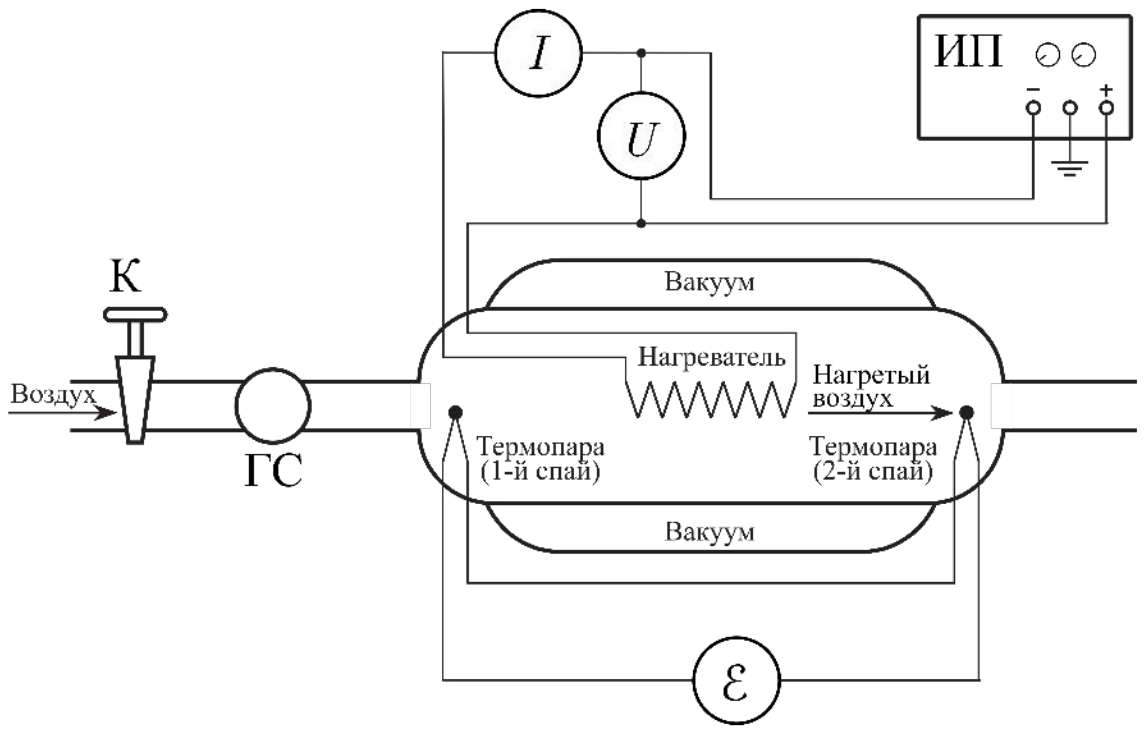
\includegraphics[scale=0.2]{asd.png}
\end{figure}
\section*{Теоретическая часть}
Измерение теплоёмкости тел обычно производится в калориметрах, т. е. в
сосудах, обеспечивающих теплоизоляцию исследуемого тела от внешней
среды. При этом регистрируется изменение его температуры $dT$ в зависимости от количества тепла $\delta Q$, полученного телом от некоторого нагревательного элемента внутри калориметра. Теплоёмкость тела в некотором процессе определяется как их отношение:
\begin{align}
	C = \frac{\delta Q}{dT}.
\end{align}
Надёжность измерения определяется, в основном, качеством калориметра.
Необходимо, чтобы количество тепла, затрачиваемое на нагревание исследуемого тела, существенно превосходило тепло, расходуемое на нагревание самого калориметра, а также на потери тепла из установки. При измерении теплоёмкости газов эти требования выполнить довольно трудно — масса газа в калориметре и, следовательно, количество тепла, идущее на его нагревание, как правило, малы. Для увеличения количества нагреваемого газа при неизменных размерах установки в нашей работе исследуемый газ (воздух) продувается через калориметр, внутри которого установлен нагреватель. При этом измеряются мощность нагревателя, масса воздуха, протекающего в единицу времени (расход), и приращение его температуры.

Рассмотрим газ, протекающий стационарно слева направо через
трубу постоянного сечения, в которой установлен нагревательный элемент. Пусть за некоторое
время $dt$ через калориметр прошла малая порция газа массой $dm = q dt$, где $q$ --- массовый расход газа в трубе. Если мощность нагрева равна $N$, мощность тепловых потерь на обмен с окружающей средой $N_{\text{пот}}$, то порция получила тепло $\delta Q = (N - N_{\text{пот}})dt$. С другой стороны, по определению теплоёмкости $\delta Q = c dm \Delta T$, где $\Delta T = T_2 - T_1$ --- приращение температуры газа, $c$ --- удельная теплоёмкость газа в рассматриваемом процессе. При малых расходах газа и достаточно большом диаметре трубы перепад давления на её концах мал, потому можно принять, что $P_1 \approx P_2 = P_0$, где $P_0$ --- атмосферное давление. Следовательно, в условиях опыта измеряется удельная теплоёмкость при постоянном давлении $c_p$. Таким образом, получаем
\begin{align}
	c_p = \frac{N - N_{\text{пот}}}{q \Delta T}
\end{align}

Напряжение $U$ на нагревателе и ток $I$ через него регистрируются цифровыми мультиметрами. Таким образом, мощность нагрева равна
\begin{align}
	N = UI.
\end{align}

Для измерения разности температур $\Delta T$ служит медно-константановая термопара. Один спай термопары расположен в струе воздуха, входящего в калориметр, и находится при комнатной температуре, а второй - в струе выходящего нагретого воздуха. Константановая проволка термопары расположена вдоль калориметра, а медные проводники подключены к цифровому вольтметру. Возникающая в термопаре ЭДС пропорциональна разности температур $\Delta T$ спаев:
\[
	\mathcal{E} = \beta \Delta T,	
\]
где $\beta = 40.7 \frac{\text{мкВ}}{K}$ --- чувствительность медно-константановой термопары в рабочем диапазоне температур. ЭДС регистрируется с помощью микровольтметра.

Объём воздуха, прошедшего через калориметр, измеряется газовым счётчиком ГС. Для регулировки служит кран K. Время $\Delta t$ прохождения некоторого объёма $\Delta V$ воздуха измеряется секундомером. Объёмный расход может быть найден как
\[
	q = \rho \frac{\Delta V}{\Delta t},
\]
где $ \rho $ --- плотность воздуха при комнатной температуре, которая в свою очередь может быть получена из уравнения Менделеева-Клапейрона:
\[
	\rho_0 = \frac{\mu P_0}{R T_0},
\]
где $P_0$ --- атмосферное давление, $T_0$ --- комнатная температура (в Кельвинах), $\mu = 29,0 \frac{\text{г}}{\text{моль}}$ --- средняя молярная масса (сухого) воздуха.

Учитывая особенности калориметра, следует ожидать, что мощность нагревателя расходуется не только на нагрев массы прокачиваемого воздуха, но и частично теряется за счёт нагрева внутренних стенок термостата и рассеяния тепла через торцы термостата. Можно предположить, что при небольшом нагреве $(\Delta T \ll T_0)$ мощность потерь тепла $N_{\text{пот}}$ прямо пропорциональна разности температур:
\[
	N_{\text{пот}}=\alpha\ \Delta T
\]
Следовательно, при фиксированном расходе воздуха $(q = const)$ подводимая мощность и разность температур свящаны прямой пропорциональностью $\left( \Delta T (N) \right)$ --- линейная функция).
\[
	N = (c_Pq+\alpha)\Delta T
\]

В общем случае давление
на входе может заметно превышать таковое на выходе
(например, если труба достаточно узкая и длинная). Рассмотрим течение газа более
детально, чтобы выяснить пределы применимости $P = const$. Обозначим индексом 1 параметры газа на входе в трубку, индексом 2 --- на выходе из неё. Рассмотрим область, мысленно ограниченную двумя неподвижными плоскостями слева и справа от нагревателя и применим к ней закон сохранения энергии.

Пусть за время $dt$ газ сместился слева направо на малое расстояние вдоль
трубки, такое что через левую границу прошёл газ объёмом $dV_1$m а через правую --- $dV_2$. В силу закона сохранения массы имеем
\[
	m = \rho_1 dV_1 = \rho_2 d V_2,
\]
где $dm = q dt$ --- масса газа, прошедшего через некоторое сечение трубки.
Изменение внутренней энергия газа в рассматриваемой области за счёт переноса вещества составило $dU = (u_2 - u_1)dm$, где $u_{1, 2}$ --- удельные внутренние энергии. Внешние силы совершили работу по перемещению газа $\partial A = P_1 dV_1 - P2 dV_2$, или с учётом предыдущей формулы:
\[
	\partial A = - (\frac{P_2}{\rho_2} - \frac{P_1}{\rho_1})dm.
\]
УЧтём также изменени кинетической энергии течения газа, равное $dK = \frac{1}{2}(v_2^2 - v_1^2)dm$, где $v_{1, 2}$ --- скорости течения. Наконец, пусть $\partial Q$ --- количество тепла, суммарно полученное газом в рассматриваемой области --- включая тепло от нагревателя, теплопередачу через стенки и торцы, тепловыделение при трении и т. д. В стационарном состоянии энергия газа, заполняющего калориметр, неизменна, поэтому
\[
	dU - dA + dK = \partial Q
\]
Полученное удобно записать в виде
\[
	(i_2 - i_1 + \frac{v_2^2}{2} - \frac{v_1^2}{2}) dm = \partial Q,
\]
где $i = u + \frac{P}{\rho}$ --- удельная энтальпия газа.
Это соотношение справедливо для любой стационарно текущей непрерывной среды и представляет собой обобщение известного уравнения Бернулли, учитывающее выделение и потери тепла. Оно справедливо при условии, что в системе устанавливается не только стационарное течение, но и стационарное распределение температуры. Последнее весьма важно для нашего опыта, поскольку время установления может быть довольно велико.

Если предположить, что кинетическая энергия течения мала по сравнени. с энергией нагрева ($dK \ll \partial Q$), то получим 
\[
	(i_2 - i_1) dm = \partial Q,
\]
то есть полученное газом тепло идёт на приращение его энтальпии.

В условмях опыта газ с хорошей точностью можно считать идеальным: $P / \rho = RT / \mu$, а теплоёмкость $c_p$ (или $c_v$) не зависящей от температуры. Тогда энальпия (и внутренняя энергия) газа зависит только от температуры и равна $\Delta i = c_p \Delta T$ (т. к. $\Delta u = c_V \Delta T$ и $c_p = c_v + \frac{R}{\mu}$). В таком случае, в этой лабораторной работе мы измеряем удельную теплоёмость газа при постоянном давлении.
\section*{Обработка результатов измерений}
\begin{figure}[H]
\center

\begin{tabular}{|c|c|c|c|c|c|}
\hline $P_0,\ \text{мм}.\ \text{рт}.\ \text{ст}. $ & $T_{\text{к}}, \text{K}$ & $\varphi, \%$ & $\Delta t_{max}, c$ & $\Delta V_{max},\ \text{дм}^3$ & $P_{\text{н.п.}},\ \text{кПа}$ \\\hline
 $749.3 \pm 0.5$ & $294 \pm 1$ & $81 \pm 1$ & $26.0 \pm 0.5$ & $5 \pm 0.1$ & $2.48$ \\\hline
\end{tabular}
\end{figure}
Объёмный расход для каждого из опытов вычислим по формуле:
\[
	q = \rho_0 \frac{\Delta V}{\Delta t}
\]
\[
	\rho_0 = \frac{\mu \left(P_0 - \varphi P_{\text{н. п.}} \right)}{RT_\text{к}} = 1.18 \pm 0.01\ \frac{\text{кг}}{\text{м}^3};
\]
\[
	\sigma
\]

\begin{figure}[H]
\center
\begin{tabular}{|c|c|c|c|c|c|}
\hline $\Delta t_1, c$ & $\Delta V_1, \text{дм}^3$ & $q_1, \frac{\text{г}}{c}$ & $\Delta t_2, c$ & $\Delta V_2, \text{дм}^3$ & $q_2, \frac{\text{г}}{c}$ \\\hline
 $26.0 \pm 0.5$ & $5 \pm 0.1$ & $0.192 \pm 0.03$ & $44.8 \pm 0.5$ & $5 \pm 0.1$ & $0.112 \pm 0.03$ \\\hline
\end{tabular}
\end{figure}

Посчитаем мощность нагрева $N$ и разность температур $\Delta T$ по формулам:
\[
	N = UI;
\]
\[
	\Delta T = \frac{\mathcal{E}}{\beta}.
\]
При расходе $q_1$:
\begin{figure}[H]
\center
\begin{tabular}{|c|c|c|c|c|c|c|}\hline
{} &   $\mathcal{E}, \text{мкВ}$ & $U_\text{н}, \text{В}$ & $I_\text{н}, \text{мА}$ & $\Delta t, K$ & $N,\, \text{Вт}$ & $R_\text{н},\ \text{Ом}$ \\\hline
1 &  102 &  4.44 &  155.8 &  2.506 &  0.6918 &  28.50 \\\hline
2 &  138 &  5.20 &  182.7 &  3.391 &  0.9500 &  28.46 \\\hline
3 &  174 &  5.89 &  206.7 &  4.275 &  1.2175 &  28.50 \\\hline
4 &  210 &  6.46 &  226.8 &  5.160 &  1.4651 &  28.48 \\\hline
5 &  242 &  7.00 &  245.7 &  5.946 &  1.7199 &  28.49 \\\hline
\end{tabular}
\end{figure}

При расходе $q_2$:
\begin{figure}[H]
\center
\begin{tabular}{|c|c|c|c|c|c|c|}\hline
{} &   $\mathcal{E}, \text{мкВ}$ & $U_\text{н}, \text{В}$ & $I_\text{н}, \text{мА}$ & $\Delta t, K$ & $N,\, \text{Вт}$ & $R_\text{н},\ \text{Ом}$ \\\hline
1 &   38 &  2.55 &   89.3 &  0.934 &  0.2277 &  28.55 \\\hline
2 &   75 &  3.50 &  122.9 &  1.843 &  0.4302 &  28.48 \\\hline
3 &  126 &  4.41 &  154.7 &  3.096 &  0.6822 &  28.51 \\\hline
4 &  165 &  5.08 &  178.1 &  4.054 &  0.9047 &  28.52 \\\hline
5 &  217 &  5.77 &  202.3 &  5.332 &  1.1673 &  28.52 \\\hline
\end{tabular}


\end{figure}
Построим графики зависимости $\Delta T(N)$ для каждого объёмного расхода воздуха $q$ и найдём угловые коэффициенты наклона графиков:

\begin{figure}[H]
\center
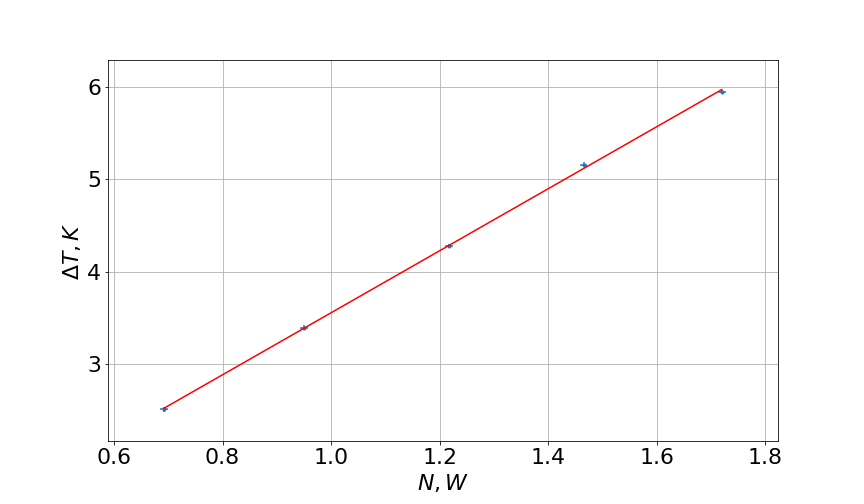
\includegraphics[scale=0.4]{q1.png}
\caption{График зависимости $\Delta T(N)$ при объёмном расходе $q_1$}
\end{figure}

\begin{figure}[H]
\center
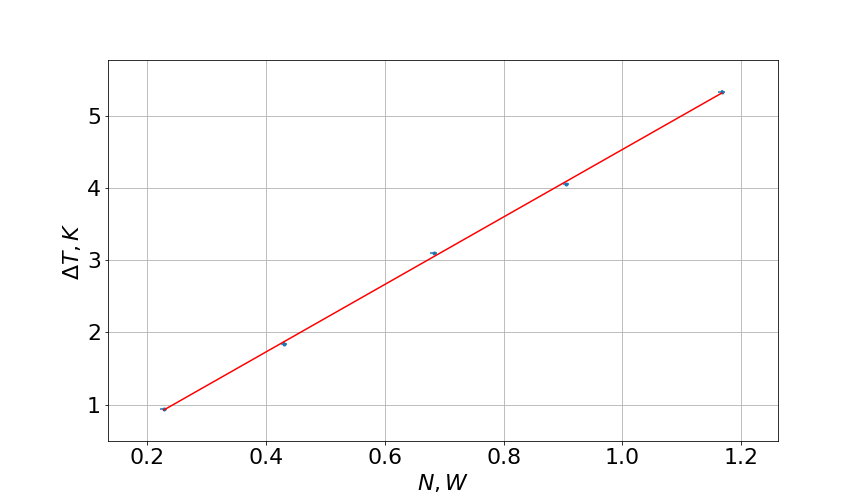
\includegraphics[scale=0.4]{q2.png}
\caption{График зависимости $\Delta T(N)$ при объёмном расходе $q_2$}
\end{figure}

Полученные зависиомсти из графиков:
\[
y_1 =k_1 x_1 + b_1;\qquad y_2 = k_2 x_2 + b_2;
\]
\[
k_1 = 3.36 \pm 0.03; \quad b_ 1 = 0.19 \pm 0.04; 
\]
\[ 
k_2 = 4.66 \pm 0.04; \quad b_ 2 = - 0.13 \pm 0.03;
\]
Найдем $\alpha$ и $c_P$, решив систему уравнений:
\[
	\left\{
		\begin{aligned}
			& c_P\, q_1 + \alpha = \frac{1}{k_1} \\
			& c_P\, q_2 + \alpha = \frac{1}{k_2}
		\end{aligned}
	\right.
\]
Путем математических преобразований получаем:
\[
\begin{aligned}
	 c_P = \frac{k_2 - k_1}{(q_1 - q_2)\, k_1\, k_2}; & \qquad  \alpha = \frac{k_2-k_1-c_P(q_1+q_2)}{2\,k_1\,k_2}. \\
	 c_P = 1038\ \frac{\text{Дж}}{\text{кг К}}; & \qquad  \alpha = 0.098\ \frac{\text{Дж}}{K} 
\end{aligned}
\]
Оценим погрешности:

\[
	\sigma_{k_1} = 0.03; \qquad \sigma_{k_1} = 0.04;
\]
\[
	\sigma_{c_P} \approx c_P \sqrt{\left(\frac{\sigma_{k_1}}{k_1}\right)^2 + \left(\frac{\sigma_{k_2}}{k_2}\right)^2} = 13
\]

\[
			\begin{aligned}
			& \fbox{$ c_P  =   1038 \pm 13 \frac{\text{Дж}}{\text{кг К}}$} \\
			& \fbox{$ \alpha = 0.098\pm 0.001\ \frac{\text{Дж}}{K} $}
			\end{aligned}
\]

\section*{Вывод}
Найденное значение молярной темлоёмкости $c_P $ с учётом погрешности и потерь тепла совпадает с табличным значением $c_{P_\text{табл}} = 1003\ \frac{\text{Дж}}{\text{кг К}}$. Мощность потерь тепла в единицу изменения температуры равна $N_\text{пот} = 0.098\ \text{Дж}$.
\end{document}